\chapter{Mathematical Background}

\section{Rayleigh Distribution} 
\label{app:rayleigh}

Let $\boldsymbol{r}$ be a vector in a two-dimensional space defined by \[\boldsymbol{r} = (x,y)\] where $x$‬ and $y$‬ represent its Cartesian coordinates. The magnitude of $\boldsymbol{r}$ would be:
\begin{equation}
    r = \sqrt{x^2+y^2}
    \label{eq-app:m_r}
\end{equation}

At the same time, let $x$ and $y$ follow the Normal Distribution located at zero ($\mu=0$) and have the same variance ($\sigma^2$): \[x \sim N(0,\sigma^2), y \sim N(0,\sigma^2)\] Their probability density function (PDF) are:
\begin{equation}
    f(x)=\frac{1}{\sigma\sqrt{2\pi}}e^{-\frac{x^2}{2\sigma^2}}, f(y)=\frac{1}{\sigma\sqrt{2\pi}}e^{-\frac{y^2}{2\sigma^2}}
    \label{eq-app:normal}
\end{equation}

When $x$ and $y$ are two fully independent variables, the joint PDF of them is:
\begin{equation}
    f(x,y)=f(x)f(y)=\frac{1}{\sigma^2 2\pi}e^{-\frac{x^2+y^2}{2\sigma^2}}
    \label{eq-app:jpdf}
\end{equation}

To calculate the PDF of the magnitude $r$, we need to transform $x$ and $y$ to Polar Coordinate:\[x=r\cos{\theta},y=r\sin{\theta}\]
where $r\geq0$ and $\theta \in [0, 2\pi)$‬‬.

When doing coordinate transformation, we must multiply by the absolute value of the Jacobian determinant, $|J|$‬. The Jacobian matrix of the transformation from $(x,y)$ to $(r,\theta)$ is:
\begin{equation}
|J| = \begin{vmatrix} \frac{\partial x}{\partial r} & \frac{\partial x}{\partial \theta} \\ \frac{\partial y}{\partial r} & \frac{\partial y}{\partial \theta} \end{vmatrix} = \begin{vmatrix} \cos\theta & -r\sin\theta \\ \sin\theta & r\cos\theta \end{vmatrix} = r(\cos^2\theta + \sin^2\theta) = r
\label{eq-app:jacob}
\end{equation}

Then we can get the joint PDF of $r$ and $\theta$ by combination \ref{eq-app:jpdf} and \ref{eq-app:jacob}:
\begin{equation}
    f(r,\theta) = f(r\cos{\theta},r\sin{\theta})\cdot|J| = \frac{1}{2\pi\sigma^2}e^{-\frac{r^2}{2\sigma^2}} \cdot r
    \label{eq-app:jpdf-polar}
\end{equation}

Consequently, the PDF of $r$ is:
\begin{equation}
    f(r) = \int^{2\pi}_{0} f(r,\theta) = \int^{2\pi}_{0} \frac{1}{2\pi\sigma^2}e^{-\frac{r^2}{2\sigma^2}} \cdot r d\theta = \frac{r}{\sigma^2}e^{-\frac{r^2}{2\sigma^2}}
    \label{eq-app:jpdf_ray}
\end{equation}
where $r$ is follow the Rayleigh Distribution.

The PDF of Rayleigh Distribution is:
\begin{equation}
    f(x) = 
    \begin{cases}
        \frac{x}{\sigma^2}e^{-\frac{x^2}{2\sigma^2}}, & x \geq 0 \\
        0, & x < 0
    \end{cases}
    \label{eq-app:pdf_ray}
\end{equation}

\begin{figure}[htbp]
    \centering
    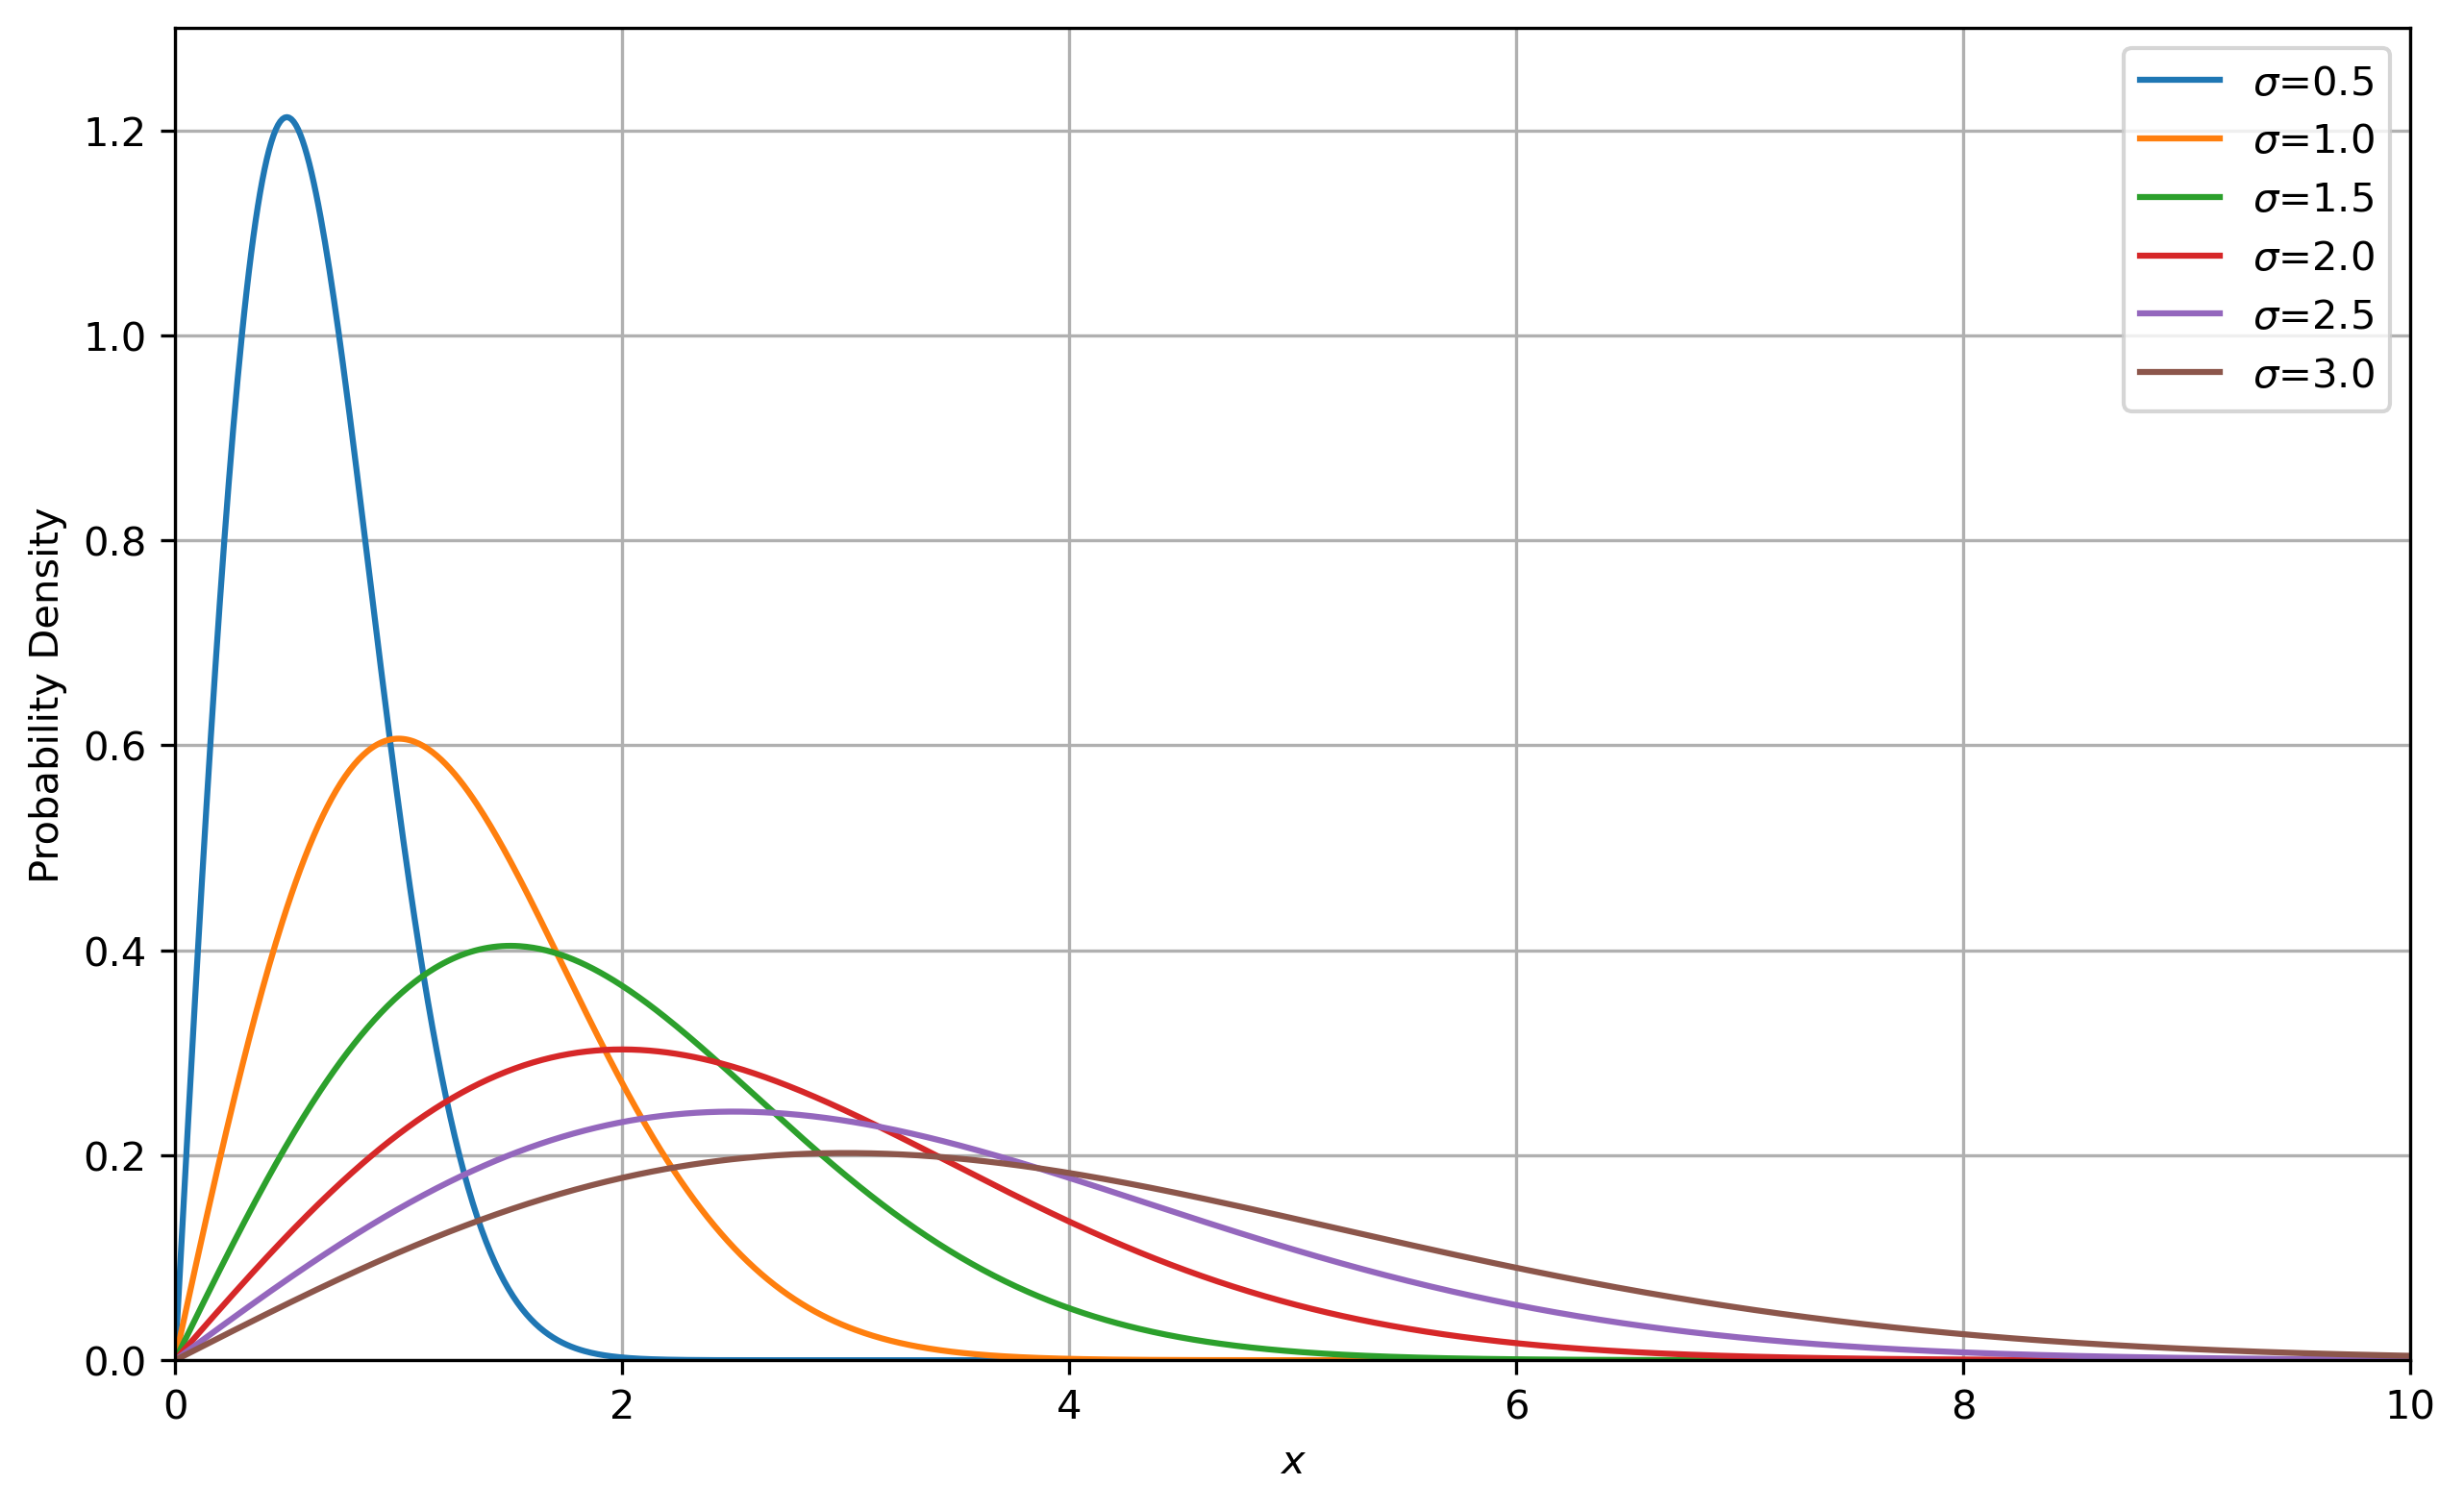
\includegraphics[width=0.9\linewidth]{paper//figs//math/rayleigh_distributions.png}
    \caption{Probability Density Function of Rayleigh Distribution with different standard variance ($\sigma$).}
    \label{fig-app:ray_pdf}
\end{figure}